\documentclass[12pt]{article}
\usepackage{coursenote}

\begin{document}
\title{STAT 401 Chapter 2.1--2.5, 2.10}
\maketitle

\section{Some probability}

Appendices A.3, A.4.

$X$ and $Y$ are random variables.\\
$a$ and $b$ are constants.

\subsection{Expected value}

Discrete variable $X$:
\[
E[X] = \sum_{i=1}^n x_i \, p(x_i)
\]
were $x_1,\dotsc,x_n$ are all possible values of $X$,
and $p(x_i)$ is the probability of $x_i$.

Continuous variable $X$:
\[
E[X] = \int_{-\infty}^{\infty} x f(x)\diff x
\]
where $f(x)$ is the pdf.

\subsection{Variance}

\[
\var(X) = E\bigl[\bigl(X - E[X]\bigr)^2\bigr]
\]

Discrete variable $X$:
\[
\var(X) = \sum_{i=1}^n \bigl(x_i - E[X]\bigr)^2\, p(x_i)
\]

Continuous variable $X$:
\[
\var(X) = \int_{-\infty}^{\infty} \bigl(x - E(X)\bigr)^2 f(x)
    \diff x
\]


\subsection{Covariance}

\[
\cov(X,Y) = E\bigl[\bigl(X - E[X]\bigr)\bigl(Y - E[Y]\bigr)\bigr]
\]
One can see that $\var(X) \equiv \cov(X,X)$.

Discrete variables $X$, $Y$:
\[
\cov(X,Y) = \sum_{i=1}^n
    \bigl(x_i - E[X]\bigr)
    \bigl(y_i - E[Y]\bigr)
    \,p(x_i, y_i)
\]
where $(x_1,y_1),\dotsc,(x_n,y_n)$ are all possible values
of the vector $(X,Y)$,
and $p(x_i,y_i)$ is the probability of $(x_i,y_i)$.

Continuous variables $X$, $Y$:
\[
\cov(X,Y) = \int_{-\infty}^{\infty}
    \int_{-\infty}^{\infty}
        \bigl(x - E(X)\bigr)
        \bigl(y - E(Y)\bigr)
        \, f(x,y)
        \diff x \diff y
\]
where $f(x,y)$ is the pdf.

\subsection{Properties}

\begin{enumerate}
\item
    \[ \var\{X\} = E\{X^2\} - \bigl(E\{X\}\bigr)^2 \]

\exercise Prove this.

\item
    \[ X, Y \text{ independent } \Rightarrow \cov\{X,Y\} = 0 \]
    If $X$ and $Y$ are jointly normal, then
    \[ X, Y \text{ independent } \Leftrightarrow \cov\{X,Y\} = 0\]
\item
    \[ E[aX + b] = aE[x] + b \]
\item
    \[ E\biggl[ \sum_{i=1}^n a_i X_i \biggr]
        = \sum_{i=1}^n a_i\, E[X_i] \]

    Interpretation: $E[\cdot]$ is a linear operator.
\item
    \[ \var(a) = 0 \]
    \[ \var(X + b) = \var(X) \]
    \[ \var(aX + b) = a^2\var(X) \]

\item
    \[ \begin{split}
    \var\biggl( \sum_{i=1}^n a_i X_i \biggr)
        &= \sum_{i=1}^n \sum_{j=1}^n a_i\, a_j \cov(X_i, X_j) \\
        &= \sum_{i=1}^n a_i^2 \var(X_i)
            + \sum_{\substack{i, j\\i\ne j}}
                a_i\, a_j \cov(X_i, X_j)
    \end{split}
    \]
\item $X_i$'s are independent $\Rightarrow$
    \[ \var\biggl( \sum_{i=1}^n a_i X_i \biggr)
        = \sum_{i=1}^n a_i^2 \var(X_i)
    \]
\item
    \[
    \cov\biggl( \sum_{i=1}^n a_i X_i,\, \sum_{j=1}^m b_j Y_j \biggr)
        = \sum_{i=1}^n \sum_{j=1}^m a_i\, b_j \cov(X_i, Y_j)
    \]
\end{enumerate}

\subsection{Some univariate distributions}

\subsubsection{\fbox{Normal}}

Standard normal, often denoted by $Z$.
\[
f(z) = \frac{1}{\sqrt{2\pi}} e^{-z^2/2}
\]
On $(-\infty, \infty)$. Symmetric about 0.
Single mode, at 0.

The normal distribution is fully described by it mean and variance.

\emph{A linear combination of normal variables is a normal variable.}

From standard normal to non-standard normal:
\[ Z \sim N(0,1) \Rightarrow X = aZ + b \sim N(b, a^2) \]
So see this,
first note that $X$ is a linear function of the normal variable $Z$,
hence $X$ is normal.
Then we only need to work out the mean and variance of $X$.
Second, we have
$E[X] = aE[Z] + b = b$ and
$\var(X) = a^2\var(Z) = a^2$.

Similarly,
from non-standard normal to standard normal (standardization):
\[ X \sim N(a, b^2) \Rightarrow Z = \frac{X - a}{b} \sim N(0,1) \]


\subsubsection{\fbox{$\chi^2$}}

The sum of
\emph{squared} \emph{independent} standard normal variables
is a $\chi^2$ variable:

\parbox{.45\textwidth}{%
\[
z_1^2 + z_2^2 +\dotsb+z^2_\nu \sim \chi^2_\nu
\]
}\parbox{.54\textwidth}{%
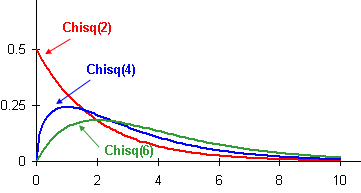
\includegraphics[width=.54\textwidth]{fig_chi2.png}
}

$\nu$: degrees of freedom. Non-negative.

\subsubsection{\fbox{$t$}}

A $t$ variable is constructed from
\emph{independent} standard normal variable $z$
and $\chi^2_\nu$ variable:

\parbox{.40\textwidth}{%
\[
\frac{z}{\sqrt{\chi^2_{\nu} / \nu}} \sim t_\nu
\]%
}\parbox{.59\textwidth}{%
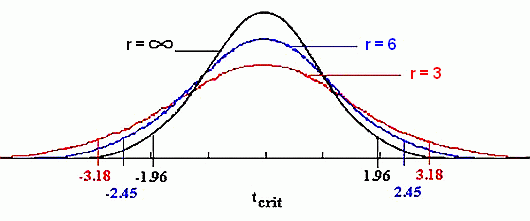
\includegraphics[width=.58\textwidth]{fig_t.png}
}

$\nu$: degrees of freedom.
On $(-\infty, \infty)$. Symmetric about 0.
Single mode, at 0.
Similar to, but ``fatter'' than standard normal.

\subsubsection{\fbox{$F$}}

The quotient of two \emph{independent} $\chi^2$ variables
is a $F$ variable:

\parbox{.40\textwidth}{%
\[
\frac{\chi^2_{\nu_1}}{\nu_1} \Bigm/
    \frac{\chi^2_{\nu_2}}{\nu_2}
\sim
F_{\nu_1, \nu_2}
\]
}\parbox{.59\textwidth}{%
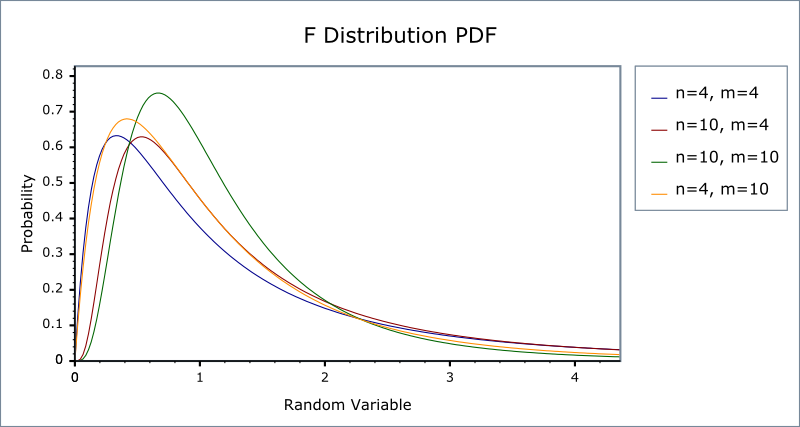
\includegraphics[width=.58\textwidth]{fig_F.png}
}

$\nu_1$, $\nu_2$: degrees of freedom (the order of the two matters).
Non-negative.

The square of a $t$ variable is a $F$ variable:
\[
t_\nu^2 \sim F_{1,\nu}
\]

\newpage

\section{Sampling distributions of $\hat{\beta}_0$, $\hat{\beta}_1$, $S^2$}

Continue our analysis of the simple regression model with normal errors
$\epsilon_i \overset{iid}{\sim} N(0, \sigma^2)$.

We will make \emph{inferences} about an unknown parameter,
such as $\beta_1$, based on data.
This is usually carried out starting with an \emph{estimator} of the
parameter,
such as
\[
\hat{\beta}_1
= \frac{\sum \bigl(X_i - \overline{X}\bigr)\bigl(Y_i - \overline{Y}\bigr)}
        {\sum \bigl(X_i - \overline{X}\bigr)^2}
.
\]
An estimator is a \emph{statistic} (that is, function) of the data.
The value of the estimator (that is, the estimate) changes with the
particular data, which are assumed to have arisen
according to our \emph{model} which contains random components.
As we obtain another set of data under identical conditions,
the random mechanism will work to give rise to a different dataset.
Each of such datasets is called a \emph{sample}.
The value of the estimator changes from sample to sample,
hence the estimator is a \emph{random variable}.
The distribution of this random variable is
called its \emph{sampling distribution}.

In the context of linear regression,
\emph{re-sampling} entails getting a new set of $Y_i$ values,
keeping the set of $X_i$ values unchanged.

Always remember that $\hat{\beta}_0$
and $\hat{\beta}_1$ are \emph{random variables}.
(Their values vary as we re-sample the $Y$'s.)
We'll use the upper-case $S^2$ to mean MSE, \ie $\text{SSE}/(n-2)$,
emphasizing its being a \emph{variable} as well,
and use $s^2$ for its value given by a particular data set.

\subsection{$\hat{\beta}_0$ and $\hat{\beta}_1$ are linear estimators}

\begin{equation}
\begin{split}
\hat{\beta}_1 = \frac{S_{xy}}{S_{xx}}
    &= S_{xx}^{-1} \sum_{i=1}^n (x_i - \overline{x})(Y_i - \overline{Y})
\\
    &= S_{xx}^{-1} \biggl(
        \sum_{i=1}^n (x_i - \overline{x}) \,Y_i
        - \overline{Y} \sum_{i=1}^n (x_i - \overline{x})
        \biggr)
\\
    &= S_{xx}^{-1} \sum_{i=1}^n (x_i - \overline{x}) \,Y_i
\\
    &= \sum_{i=1}^n k_i Y_i
,
\end{split}
\end{equation}
where $k_i = (x_i - \overline{x}) / S_{xx}$
and we have used the factor
$\sum_{i=1}^n (x_i - \overline{x}) = 0$.

We have used different cases for $X$ and $Y$ to emphasize that
the $x$'s are constants but $Y$'s are variables.

Conclusion:
$\hat{\beta}_1$ is a linear function of the $Y$'s.

Similarly,
\begin{equation}
\begin{split}
\hat{\beta}_0 = \overline{Y} - \hat{\beta}_1 \overline{x}
    &= \frac{\sum_i Y_i}{n} - \overline{x}\sum_i k_i Y_i
\\
    &= \sum_i \Bigl(\frac{1}{n} - \overline{x}k_i\Bigr) Y_i
,
\end{split}
\end{equation}
which is another linear function of the $Y$'s.

\exercise
Prove the following properties of the $k_i$'s (page 42):\\
(1) $\sum k_i = 0$;\\
(2) $\sum k_i x_i = 1$;\\
(3) $\sum k_i^2 = 1 / S_{xx}$.

\subsection{Sampling distributions}

\alert[Theorem]%
1. $\hat{\beta}_1 \sim N(\beta_1, \sigma^2 / S_{xx})$.\\[3pt]
2. $\hat{\beta}_0 \sim N\bigl(\beta_0,
        \bigl(1/n + \overline{x}^2/S_{xx}\bigr)
        \sigma^2\bigr)$.\\[3pt]
3. $\cov(\hat{\beta}_0, \hat{\beta}_1) = -\overline{x} \sigma^2 / S_{xx}$.\\[3pt]
4. $S^2$ is independent of $\hat{\beta}_0$ and $\hat{\beta}_1$.\\[3pt]
5. $\frac{(n-2)S^2}{\sigma^2} \sim \chi^2_{n-2}$.
    (Note $(n-2)S^2$ is SSE.)\\[3pt]
6. $E(S^2) = \sigma^2$.


\textbf{Partial proof}:

\indentblock{%
Extensively use the model assumptions that
the $Y_i$'s are independent normal variables,
as well as the properties of the $k_i$'s.

1.

Because $\hat{\beta}_1$ is a linear function of the normal variables $Y_i$,
$\hat{\beta}_1$ is normal.
(The independence between the $Y_i$ is not needed for this statement.)

\[
E(\hat{\beta}_1)
= \sum_i k_i E(Y_i)
= \sum_i k_i (\beta_0 + \beta_1 x_i)
= \beta_0 \sum_i k_i + \beta_1 \sum_i k_i x_i
= \beta_1
\]

\[
\var(\hat{\beta}_1)
= \sum_i k_i^2 \var(Y_i)
= \sigma^2 \sum_i k_i^2
= \frac{\sigma^2}{S_{xx}}
\]

2.

Because $\hat{\beta}_0$ is a linear function of the normal variables $Y_i$,
$\hat{\beta}_0$ is normal.
(The independence between the $Y_i$ is not needed for this statement.)

\[
E(\hat{\beta}_0)
= \sum_i \Bigl(\frac{1}{n} - \overline{x} k_i\Bigr) E(Y_i)
= \sum_i \Bigl(\frac{1}{n} - \overline{x} k_i\Bigr)
    (\beta_0 + \beta_1 x_i)
= \Bigl(1 - \overline{x}\sum_i k_i\Bigr) \beta_0
    + \Bigl(\overline{x} - \overline{x} \sum_i k_i x_i\Bigr) \beta_1
\]

\[
\var(\hat{\beta}_0)
= \sum_i \Bigl(\frac{1}{n} - \overline{x}k_i\Bigr)^2 \var(Y_i)
= \sigma^2 \sum_i \Bigl(\frac{1}{n^2} - \frac{2\overline{x}k_i}{n} +
    \overline{x}^2 k_i^2\Bigr)
= \sigma^2 \Bigl(\frac{1}{n} - \frac{2\overline{x}}{n}\sum_i k_i
    + \overline{x}^2 \sum_i k_i^2\Bigr)
\]

3.

\[
\begin{split}
\cov(\hat{\beta}_0, \hat{\beta}_1)
&= \sum_i \sum_j
    \Bigl(\frac{1}{n} - \overline{x}k_i\Bigr)\,
    k_j\,
    \cov(Y_i, Y_j)
\\
&= \sum_i \Bigl(\frac{1}{n} - \overline{x} k_i\Bigr) k_i \var(Y_i)
\\
&= \sigma^2 \Bigl(\frac{1}{n} \sum_i k_i - \overline{x}\sum_i k_i^2\Bigr)
\end{split}
\]
where we have used
$\cov(Y_i, Y_j) = 0$ if $i\ne j$.

4. Do not worry about the proof.

5. Do not worry about the proof.

6.

From $\frac{(n-2)S^2}{\sigma^2} \sim \chi^2_{n-2}$, we have
(per a property of the $\chi^2$ distribution)
\[
E\biggl(\frac{(n-2)S^2}{\sigma^2}\biggr) = n - 2
\]
hence
\[
E(S^2) = \sigma^2
\]
}


\alert
Not only $\hat{\beta}_0$ and $\hat{\beta}_1$ are unbiased,
but their sampling variances are the smallest among
linear, unbiased estimators of $\beta_0$ and $\beta_1$.

\alert[Proposition]%
1. $\frac{\hat{\beta}_1 - \beta_1}{S_{\hat{\beta}_1}} \sim t_{n-2}$, where
$S_{\hat{\beta}_1} = \sqrt{S^2 / S_{xx}}$.\\
2. $\frac{\hat{\beta}_0 - \beta_0}{S_{\hat{\beta}_0}} \sim t_{n-2}$, where
$S_{\hat{\beta}_0} = \sqrt{\bigl(1/n + \overline{x}^2/S_{xx}\bigr) S^2}$.

Comparing $\sigma^2_{\hat{\beta}_1}$ (the variance of the
sampling distribution of $\hat{\beta}_1$)
and $S_{\hat{\beta}_1}$,
we see that
$S^2_{\hat{\beta}_1}$ is $\sigma^2_{\hat{\beta}_1}$
with the unknown $\sigma^2$ replaced by its estimator
$S^2$.

\textbf{Proof}

\indentblock{%
Making use of
$\sigma^2_{\hat{\beta}_1} = \sigma^2 / S_{xx}$ and
$S^2_{\hat{\beta}_1} = S^2 / S_{xx}$,
write
\[
\frac{\hat{\beta}_1 - \beta_1}{S_{\hat{\beta}_1}}
= \frac{(\hat{\beta}_1 - \beta_1) / \sigma_{\hat{\beta}_1}}
    {S_{\hat{\beta}_1} / \sigma_{\hat{\beta}_1}}
= \frac{(\hat{\beta}_1 - \beta_1) / \sigma_{\hat{\beta}_1}}
    {\sqrt{S^2 / \sigma^2}}
= \frac{(\hat{\beta}_1 - \beta_1) / \sigma_{\hat{\beta}_1}}
    {\sqrt{\frac{(n-2) S^2 / \sigma^2}{n-2}}}
\]
Denote the above by $U / \sqrt{V / (n-2)}$.
Notice $U \sim N(0,1)$ and $V \sim \chi^2_{n-2}$.
If $U$ and $V$ are independent,
then $U / \sqrt{V/(n-2)}$ is a $t_{n-2}$ variable.
(See ``Some probability''.)
The independence is true, following item~4 of the theorem above.

Proof for item~2 is similar.
}

\alert
We will see this pattern of going from $N(0,1)$ to $t$ again.
If $X \sim N(\mu, \sigma^2)$, then $\frac{X - \mu}{\sigma} \sim N(0,1)$.
If we replace $\sigma$ by an estimate, say $s$, then often
$\frac{X - \mu}{s} \sim t$ (of a suitable degrees of freedom).
This makes good sense:
(1) An estimate of $\sigma$ introduces more uncertainties, making
$\frac{X - \mu}{s}$ more variable than $\frac{X - \mu}{\sigma}$.
Incidentally, a $t$ distribution is ``fatter'' than $N(0,1)$.
(2) On the one hand,
as $n$ increases, the estimate $s$ should become steadily close to
$\sigma$, hence $\frac{X - \mu}{s}$ approaches becomes more and more
like a standard variable.
On the other hand, the $t$ distribution approaches $N(0,1)$
as its ``degree of freedom'' increases.


\newpage

\section{Review of confidence interval and hypothesis test}

(See handout \texttt{ch02b.pdf} for additional reading.)

We use $\beta_1$ and $\hat\beta_1$ as examples
to review the concepts of confidence interval and hypothesis test.
To begin with,
we know $\hat\beta_1$ is an estimator of the unknown parameter
$\beta_1$,
and the sampling distribution of $\hat\beta_1$ is
$N(\beta_1, \sigma^2/S_{xx})$.
This is an unbiased estimator because
$E(\hat\beta_1) = \beta_1$.
Given the unbiasedness,
the sampling variance indicates how good
an estimator it is.
(The smaller the sampling variance, the better.)

\subsection{Confidence interval}

$\hat\beta_1$ provides a \emph{point estimate},
\ie a single value.
However, this single value is essentially guaranteed to
be different from the true value $\beta_1$
(although we hope it gets close).
In contrast,
a \emph{confidence interval} (CI)
is an interval constructed such that it
contains the true value of the parameter with a specified
percentage (say 95\%)
if we were to re-sample the data
and re-construct the CI (which would vary with the data)
many, many times.

The ``capture'' percentage (95\%, say)
is called the ``confidence level''.
Let $\alpha = 0.05$,
then $0.95 = 1 - \alpha$ is the ``degree of confidence'' or
``confidence coefficient'',
and $95\%$ is the ``confidence level''.
We will speak of
``constructing a CI at the 95\% confidence level''
or
``constructing a 95\% CI''.

Suppose $\sigma^2$ is known,
hence the sampling variance $\sigma^2_{\hat\beta_1} = \sigma^2/S_{xx}$
is known.

Let
\[
\Delta = z_{\alpha/2}\, \sigma_{\hat\beta_1}
\]
where
$z_{\alpha/2}$ is such that
$P(Z > z_{\alpha/2}) = \alpha/2$
for the standard normal variable $Z$.
In $\texttt{R}$ we find
$z_{0.025} = \text{\texttt{qnorm}}(0.975) = 1.96$.

Then,
\begin{equation}\label{eq:CI-1}
\begin{split}
&P(\beta_1 - \Delta < \hat\beta_1 < \beta_1 + \Delta)
\\
&= 2\, P(\beta_1 < \hat\beta_1 < \beta_1 + \Delta)
\\
&= 2\, P\biggl(\frac{\beta_1 - \beta_1}{\sigma_{\hat\beta_1}}
    < \frac{\hat\beta_1 - \beta_1}{\sigma_{\hat\beta_1}}
    < \frac{\beta_1 + \Delta - \beta_1}{\sigma_{\hat\beta_1}}
    \biggr)
\\
&= 2\, P\bigl(0 < Z < z_{\alpha/2}\bigr)
\\
&= 2\, (0.5 - \alpha/2)
\\
&= 1 - \alpha\quad (=0.95)
\end{split}
\end{equation}
Note that
$\frac{\hat\beta_1 - \beta_1}{\sigma_{\hat\beta_1}}$
is a standard normal variable ($Z$)
because
$\hat\beta_1 \sim N(\beta_1, \sigma^2_{\hat\beta_1})$.

The relation~(\ref{eq:CI-1}) says that
if we sample $\hat\beta_1$
(that is, re-sample data $Y$ and calculate $\hat\beta_1$)
repeatedly, then in roughly 95\% of the repetitions
the estimate $\hat\beta_1$ falls between
$\beta_1 - \Delta$ and $\beta_1 + \Delta$.

However, we don't know $\beta_1$,
and our goal is not to say how $\hat\beta_1$ behaves but to
say something about $\beta_1$.

The probability statement~(\ref{eq:CI-1}), that is,
$P(\beta_1 - \Delta < \hat\beta_1 < \beta_1 + \Delta)
= 0.95$,
can be re-phrased as
\begin{equation}\label{eq:CI-2}
P(\hat\beta_1 - \Delta < \beta_1 < \hat\beta_1 + \Delta)
= 0.95.
\end{equation}
This statement holds, because
the relations
\[
\hat\beta_1 - \Delta < \beta_1 < \hat\beta_1 + \Delta
\]
and
\[
\beta_1 - \Delta < \hat\beta_1 < \beta_1 + \Delta
\]
are equivalent.

How can we interpret~(\ref{eq:CI-2})?

We can not say something like this:
In repeated sampling of $\hat\beta_1$,
95\% of the time $\beta_1$ falls between
$\hat\beta_1 - \Delta$ and $\hat\beta_1 + \Delta$.
That sounded like $\beta_1$ is changeable,
and it could ``fall'' somewhere.
We know $\beta_1$ is fixed (although unknown).
It sits somewhere still;
it won't ``fall'' here in this sampling and there in another sampling.

Instead, we say this:
In repeated sampling of $\hat\beta_1$
and with the interval
$(\hat\beta_1 - \Delta,\, \hat\beta_1 + \Delta)$
constructed in each sampling,
95\% of the time the interval \emph{contains} the true value of
$\beta_1$.

In reality we have just one dataset and one value of $\hat\beta_1$
(let's write this value as $b_1$).
With this single estimate,
we build an interval $(b_1 - \Delta,\, b_1 + \Delta)$,
and \emph{call it the 95\% confidence interval for $\beta_1$}.
We don't have another dataset (with the same set of $X$'s),
hence we can't ``re-sample $\hat\beta_1$''.
The one interval
$(b_1 - \Delta,\, b_1 + \Delta)$
either contains $\beta_1$ or it does not;
it makes no sense to say ``it contains $\beta_1$ with probability
0.95''.
(Only when we have many, we can say ``95\% of them...'').
Therefore,
we interpret the CI with the rhetoric
``If we were able to re-sample and repeat..., then with 0.95 probability
the interval would contain the true value.''
The logic is,
since we happened to have got this dataset,
it is just like one of the samples that we could randomly draw;
and now we follow the same recipe to construct the interval,
there is a good chance that this interval does contain the true value of
$\beta_1$.

Note that $\Delta$ is a known value because we assumed
$\hat\beta_1$ is unknown.
(In reality we don't know $\sigma^2$, hence some adjustment is
necessary.)

\subsection{Hypothesis tests}

\subsubsection{Hypothesis}

Hypothesis is a statement about an
unknown parameter, say $\beta_1$, for example,
$\beta_1 = 1$; $5.2 < \beta_1 < 5.8$; $\beta_1 > 0$.

A ``null'' hypothesis, $H_0$,
is a statement that is taken by default unless
sample data provide \emph{strong} evidence against it.
An ``alternative'' hypothesis, $H_a$, is the opposite of $H_0$.

A hypothesis test procedure looks into the sample data and
determines whether there is
\emph{strong} evidence that $H_0$ should be \emph{rejected}.

There are two possible conclusions of a test:\\
(1) \emph{reject} $H_0$;\\
(2) \emph{fail to reject} $H_0$.

Note, we do not say \emph{accept} $H_0$;
it's a lack of disproof, which is not the same as proof.
We do not say ``we believe $H_0$ is true''.
We're not sure about that; it's just that evidence against it is not
strong enough (by a prescribed criterion).

In this course, we always take $H_0$ to be an equality to
a particular number, say $\beta_{1*}$:\\
$H_0$: $\beta_1 = \beta_{1*}$

$H_a$ has three possible forms:\\
$H_a$: $\beta_1 > \beta_{1*}$\\
$H_a$: $\beta_1 < \beta_{1*}$\\
$H_a$: $\beta_1 \ne \beta_{1*}$


\subsubsection{Test procedure}

Take a function of the sample data, say $T$, called ``test statistic''.
(Any function of the sample data is called a ``statistic''.)
For example $\max(y_1,\dotsc,y_n)$, $\overline{y}$, etc.
This $T$ is a deliberate choice such that it is connected with $\beta_1$
and $H_0$.

We identify a \emph{rejection region}, i.e.\@ a set of values
(discrete numbers or interval). Let's call it $R$.

Procedure of a test:
\begin{enumerate}
\item Define a test statistic $T$ and the rejection region $R$.
\item Calculate the value of $T$ using the sample data.
\item Draw a conclusion:\\
reject $H_0$ if $T \in R$; do not reject $H_0$ if $T \notin R$.
\end{enumerate}

Take the $\beta_1$ example.
We know the estimator $\hat\beta_1$ has sampling distribution
$N(\beta_1, \sigma^2/S_{xx})$.
Suppose $\sigma^2$, hence $\sigma^2_{\hat\beta_1}$, is known.

How do we define a rejection region $R$?

This depends on how safe (conservative) we want our conclusion to be.
There is always a chance to be wrong (otherwise there is no problem of a
``hypothesis'').
Our definition of the rejection region is dictated by
what kind of mistakes we try to avoid and
what kind of mistakes are less devastating,
and considerations like that.


\definition%
\emph{Type I error}:
reject $H_0$ but it's a mistake (in fact $H_0$ is true).
\emph{Type II error}:
do not reject $H_0$ but it's a mistake (in fact $H_0$ is false).

Suppose $H_a$ is $\beta_1 \ne \beta_{1*}$.
This is called a ``two-sided'' test.
We control the chance of making a type~I error.
Specifically,
we will define a rejection region such that the probability of making a
type~I error is $\alpha = 0.05$.
(This $\alpha$ is called the ``significance level''.)
Like the concept of confidence interval,
this probability $\alpha$ has to be understood in a
``repeatable experiment'' setting.
Suppose we could re-sample data $Y$.
With each re-sampling, we determine $R$ and draw a conclusion.
In many such repetitions, we require our recipe of reaching a conclusion
(the center piece of which is how to determined $R$) is such that
at most 5\% of the time the conclusion is wrong.

Suppose we simply take $\hat\beta_1$ as the test statistic.
(This is valid because $\hat\beta_1$ is a function of the sample data,
hence a statistic.)
How should we choose the rejection $R$?

Let's ponder again how we draw a conclusion and when we make a type~I
error---%
We make a type~I error when $H_0$ is true but we reject it,
and we reject it only when $\hat\beta_1 \in R$.
Note that, to control type~I error,
we only need to care about the situation where
$H_0$ is actually true,
and in this situation we make a mistake
if and only if the calculated $\hat\beta_1$ falls in $R$.
To make the probability of this mistake 0.05,
we must have $P(\hat\beta_1 \in R) = 0.05$.

In the ``confidence interval'' section we have seen that
\[
P(\beta_1 - \Delta < \hat\beta_1 < \beta_1 + \Delta) = 1 - \alpha
\]
in other words,
\[
P(\hat\beta_1 < \beta_1 - \Delta \text{ or } \hat\beta_1 > \beta_1 + \Delta)
= \alpha \quad(= 0.05)
\]
Now we are assuming $\beta_{1*}$ is indeed
the true $\beta_1$ value.
Replacing $\beta_1$ in the above by $\beta_{1*}$, we define
\[
R = (-\infty, \beta_{1*} - \Delta) \cup
    (\beta_{1*} + \Delta, \infty)
\]

Therefore the \emph{decision rule} is
\\
\texttt{Reject $H_0$ if $\hat\beta_1 \in R$.}\\
or equivalently,
\\
\texttt{Reject $H_0$ if $|\hat\beta_1 - \beta_{1*}| > \Delta$.}

When actually conducting the test,
we should replace $\hat\beta_1$ by its actual value $b_1$
that is provided by the data.

Equivalently,
we may choose
\[
T = \frac{\hat\beta_1 - \beta_{1*}}{\sigma_{\hat\beta_1}}
\]
to be the test statistic.
Then the rejection region becomes
\[
R = (-\infty, -z_{\alpha/2}) \cup (z_{\alpha/2}, \infty)
\]
The decision rule becomes
\\
\texttt{Reject $H_0$ if $|T| > z_{\alpha/2}$.}

Another try to understand the logic in the test procedure---%
Under the assumption that
$\beta_1 = \beta_{1*}$, a low-probability event
(\ie $T \in R$) has happened.
Now we (1) have sound probability theory
and (2) do not think the only dataset we have is a strange thing.
There is a contradiction here,
because the observed $T$ is a rare event.
We argue that the cause of the awkward situation is the assumption---%
that $\beta_1 = \beta_{1*}$.
We reject the assumption and conclude that
the true $\beta_1$ is some other value.
Starting with that true value (if we knew it)
the calculated $T$ would not be a rare event
(hence our dataset is not a statistically rare observation).

To recap,
\emph{the significance level, $\alpha$,
is the probability of making type-I error.}
$\alpha$ is specified by us.
It affects the value of $\Delta$, hence
the rejection region, through the requirement
$P(\hat\beta_1 \in R) = \alpha$.

In contrast,
the probability of type~II error is not in our control.
In fact, to calculate it requires knowing the true value of $\beta_1$.

\subsubsection{P value}

Assuming $H_0: \beta_1 = \beta_{1*}$ is true,
we can examine the relative standing of the observed estimator,
$b_1$, in the sampling distribution of $\hat\beta_1$.
Suppose $b_1 > \beta_{1*}$.
Let
\[
p_1
= P(\hat\beta_1 > b_1)
= P\biggl(\frac{\hat\beta_1 - \beta_{1*}}{\sigma_{\hat\beta_1}}
    > \frac{b_1 - \beta_{1*}}{\sigma_{\hat\beta_1}}\biggr)
= P\biggl(Z > \frac{b_1 - \beta_{1*}}{\sigma_{\hat\beta_1}}\biggr)
\]
where $Z$ is the standard normal variable
and $b_1$, $\beta_{1*}$, and $\sigma_{\hat\beta_1}$
are all known values.
Therefore $p_1$ can be calculated.
This value is the probability in (imagined) repeated samplings
that $\hat\beta_1$ is more distant from $\beta_{1*}$
on the larger side (meaning $\hat\beta_1 > \beta_{1*}$)
than the observed value $b_1$ is from $\beta_{1*}$.

Since the alternative being considered here is two-sided,
we want the probability that $\hat\beta_1$ is farther away from
$\beta_{1*}$ than the observed $b_1$ is, on either side
(either far below $\beta_{1*}$ or far above $\beta_{1*}$),
we take
\[
p = P\bigl(|\hat\beta_1 - \beta_{1*}| > |b_1 - \beta_{1*}|\bigr)
  = 2p_1
\]
called the ``p value''.
\emph{$p$-value is the probability of obtaining a test statistic}
(here we are using $\hat\beta_1$ itself as the test statistic)
\emph{at least as extreme as the one that was actually observed.}
\emph{A small $p$ value is evidence against $H_0$},
because it indicates the actually observed test statistic
(here, $b_1$) is a rare event in its sampling distribution,
if $H_0$ is true.

In sum,
confidence interval and hypothesis test both rely on our knowing the
sampling distribution, hence being able to do certain calculations.


We may take either of the following two ways to do hypothesis test:
\begin{itemize}
\item
Find the rejection region $R$ and examine whether $T \in R$.
If yes, reject $H_0$.
\item
Calculate the $p$ value for the test statistic and compare $p$ to
$\alpha$. If $p < \alpha$, then reject $H_0$.
\end{itemize}

\newpage

\section{Inferences concerning $\beta_1$}

The ``inference'' here refers to
(1) construction of confidence intervals,
and (2) hypothesis tests.
You can also think of point estimation
(\ie getting $\hat\beta_1$) as another aspect of inference.


\textbf{If we know $\sigma^2$},
then since $\hat{\beta}_1 \sim N(\beta_1, \sigma^2_{\hat{\beta}_1})$
where $\sigma^2_{\hat{\beta}_1} = \sigma^2/S_{xx}$,
both confidence
interval and hypothesis test are based on standard normal.
For example,
the $(1-\alpha)$ CI of $\beta_1$ is
\[
(\hat{\beta}_1 - z_{\alpha/2}\sigma_{\hat{\beta}_1},\;
\hat{\beta}_1 + z_{\alpha/2}\sigma_{\hat{\beta}_1})
,
\]
where $z_{\alpha/2}$ is the ``critical value'' defined by
$P(Z > z_{\alpha/2}) = \alpha/2$
for the standard normal variable $Z$.
For a two-sided test
$H_0: \beta_1 = \beta_{1*}$ versus
$H_a: \beta_1 \ne \beta_{1*}$,
the null hypothesis would be rejected if
\[
\frac{|\hat{\beta}_1 - \beta_{1*}|}{\sigma_{\hat{\beta}_1}} > z_{\alpha/2}
.
\]

\textbf{In reality $\sigma^2$ is unknown},
and we have to use an estimate of it, $s^2$,
and use the property
$\frac{\hat{\beta}_1 - \beta_1}{S_{\hat{\beta}_1}} \sim t_{n-2}$.
The CI is then
\[
(\hat{\beta}_1 - t_{\alpha/2,\, n-2}s_{\hat{\beta}_1},\;
\hat{\beta}_1 + t_{\alpha/2,\, n-2}s_{\hat{\beta}_1})
,
\]
where $t_{\alpha/2,\, n-2}$ is the ``critical value'' defined by
$P(T > t_{\alpha/2,\, n-2}) = \alpha/2$ for the $t_{n-2}$ variable $T$.
(The textbook uses different notations for critical values.)
For the test above,
the null hypothesis would be rejected if
\[
\frac{|\hat{\beta}_1 - \beta_{1*}|}{s_{\hat{\beta}_1}}
    > t_{\alpha/2,\, n-2}
.
\]

Most often, one wants to test whether there is
significant \emph{linear association} between $X$ and $Y$.
That calls for a two-sided test with $H_0:\; \beta_{1*} = 0$.

\example
Page 46.

\subsubsection{One-sided tests}

For example,\\
$H_0$: $\beta_1 = \beta_{1*}$\\
$H_a$: $\beta_1 > \beta_{1*}$

Rejection rule:\\
$\frac{\hat{\beta}_1 - \beta_{1*}}{s_{\hat{\beta}_1}} > t_{\alpha,\, n-2}$
where
$t_{\alpha,\, n-2}$ is such that
$P(T > t_{\alpha,\, n-2}) = \alpha$
for the $t_{n-2}$ variable $T$.

For another example,\\
$H_0$: $\beta_1 \le \beta_{1*}$\\
$H_a$: $\beta_1 > \beta_{1*}$

Rejection rule is, again,\\
$\frac{\hat{\beta}_1 - \beta_{1*}}{s_{\hat{\beta}_1}} > t_{\alpha,\, n-2}$

In the last example,
we plug in the hypothesized value ($\beta_{10}$)
and calculate based on that value.
Now $\alpha$ is the probability of type-I error if
$\beta_1 = \beta_{1*}$, which is not exactly $H_0$.
(We can calculate the probability of type-I error
only if we plug in a specific number for the unknown,
that is, assuming the unknown is a certain value;
we can not plug in the interval $(-\infty, \beta_{1*}]$.)

\example \label{ex:tree}
Tree diameter ($X$) versus height ($Y$) example.
Suppose
$n = 50$, $S_{xx} = 4.0$, $b_1 = 1.2$, $b_0 = 1$,
$s^2 = 0.36$, $\overline{x} = 1$.\\
(1) Construct a 95\% CI of $\beta_1$.\\
(2) Test $H_0:\; \beta_1 = 0$ vs $H_a:\; \beta_1 \ne 0$
    with $\alpha = 0.05$.\\
(3) Test $H_0:\; \beta_1 = 1.0$ vs $H_a:\; \beta_1 \ne 1.0$
    with $\alpha = 0.01$.\\
(4) Test $H_0:\; \beta_1 \le 1.0$ vs $H_a:\; \beta_1 > 1.0$
    with $\alpha = 0.01$.


\example 1 on page 47.

\example 2 on page 47.

\bigskip
\textbf{Two procedures for hypothesis tests:}
\bigskip

\fbox{\textbf{Procedure 1}}
\begin{enumerate}
\item Choose a test statistic $T$ (whose sample distribution is known
under assumption $H_0$).
\item Determine the ``rejection region'' $R$ for the test.
(This will be related to the sampling distribution, the hypothesized
value in $H_0$, the $\alpha$ level, and the nature of $H_0$ and $H_1$,
meaning one-sided or two-sided, etc.)
\item Calculate the test statistic, $T^*$, using the data and fitted
model.
\item Check whether $T^* \in R$ and draw a conclusion:

If $T^* \in R$: reject $H_0$.\\
If $T^* \notin R$: fail to reject $H_0$.
\end{enumerate}

\fbox{\textbf{Procedure 2}}
\begin{enumerate}
\item Choose a test statistic $T$ (whose sample distribution is known
under assumption $H_0$).
\item Calculate the test statistic, $T^*$, using the data and fitted
model.
\item Calculate the $p$ value of $T^*$.
(This will be related to the sampling distribution, the hypothesized
value in $H_0$, and the nature of $H_0$ and $H_1$,
meaning one-sided or two-sided, etc.)
\item Draw a conclusion for any specified $\alpha$:

If $p \le \alpha$: reject $H_0$.\\
If $p > \alpha$: fail to reject $H_0$.
\end{enumerate}


\subsection*{Comments}

\subsubsection{1. Effects of departures from normality}

If the normality assumption about $\epsilon$ (or equivalently, $Y$)
is violated but $n$ is large, $\hat{\beta}_0$ and $\hat{\beta}_1$ are approx normal, per
\emph{Central Limit Theorem}.
The previous inference and test procedures are still usable.

\subsubsection{2. Interpretation of the ``confidence level'' and
``significance level''}

Again, $X$ is fixed and $Y$ is random.
See previous sections of this handout and
handout~\texttt{ch02b.pdf}.

\subsubsection{3. Spacing of the $X$ levels}

$\sigma_{\hat{\beta}_1}$ and $\sigma_{\hat{\beta}_0}$ are affected by the spread of
the $X$ levels as indicated by $S_{xx}$.
For $\hat{\beta}_1$, large $S_{xx}$ reduces its sampling variance.

\subsubsection{4. $\alpha$ versus $p$ value in tests}

In tests, I prefer to always report the $p$ value.
This is more useful than just reporting the conclusion
according to a specific ``significance level'' $\alpha$.
Given the $p$ value, it's up to the user to decide whether it is
``significant''.
Given the conclusion at a specific $\alpha$,
the user does not know how much ``extra room'' is left.

When reporting the $p$ value, report the $H_0$ and $H_a$ as
well. Otherwise the meaning of the $p$ value may be unclear.

\subsubsection{5. Power of tests}

Type-I error: reject $H_0$, wrongly.\\
Type-II error: accept $H_0$, wrongly.

Let\\
$P(\text{type-I error}) = \alpha$\\
$P(\text{type-II error}) = \beta$

$1 - \beta$ is called the ``power'' of the test, which is
the probability that
$H_0$ is rejected when $H_a$ is actually true (hence
rejection is the right conclusion).
Whereas the ``significance level'' $\alpha$ is controlled (specified) by
us, the power can not be known exactly, because it depends on the true
value of the unknown parameter (say $\beta_1$).

\subsubsection{6. How to obtain the critical value $t_{\alpha/2,\, n-2}$}

Method 1: look up table~B.2.

Method 2: use \texttt{R} function $\text{\texttt{qt}}(1-\alpha/2, n-2)$.


\section{Inferences concerning $\beta_0$}

Same idea as what we do for $\beta_1$.
The sampling distribution is normal; only the distribution parameters
are different.

\section{Inferences on $E(Y)$ at a specific $X$ level}

We already have a point estimator for $E(Y \given X = x_*)$; it is
\[
\hat{Y}_* = \hat{\beta}_0 + \hat{\beta}_1 x_*
.
\]
Since $\hat{\beta}_0$ and $\hat{\beta}_1$ are both random,
we want describe the uncertainty in $\hat{Y}_*$.
This needs the sampling distribution of $\hat{Y}_*$.
Since $\hat{Y}_*$ is a linear function of the \emph{normal} random
variables $\hat{\beta}_0$ and $\hat{\beta}_1$, we know $\hat{Y}_*$ is also normal.

\alert[Theorem]%
$E(\hat{Y}_*) = \beta_0 + \beta_1 x_*$\\
$\var(\hat{Y}_*) = \sigma^2
    \Bigl(\frac{1}{n} + \frac{(x_* - \overline{x})^2}{S_{xx}}\Bigr)
$

Remark on notation:
$x_*$ is any value one wishes to specify (within the scope of the observed
$x$); it may or may not be in the observed data set.
$\overline{x}$ and $S_{xx}$ are from the data set which has given rise
to the estimates $\hat{\beta}_0$ and $\hat{\beta}_1$;
they are not recalculated to include the contribution of $x_*$.

\textbf{Proof}

\[
E(\hat{Y}_*)
= E(\hat{\beta}_0 + \hat{\beta}_1 x_*)
= E(\hat{\beta}_0) + x_* E(\hat{\beta}_1)
= \beta_0 + \beta_1 x_*
\]
\[
\hat{Y}_*
= \hat{\beta}_0 + \hat{\beta}_1 x_*
= \sum \Bigl(\frac{1}{n} - \overline{x}k_i\Bigr) Y_i
 + \sum k_i Y_i x_*
= \sum \Bigl(\frac{1}{n} - \overline{x}k_i + x_* k_i\Bigr) Y_i
\]
(The $k_i$'s were introduced in section~2.1 of this note.)
Using the independence of $Y_i$, and properties of $k_i$:
\[
\var(\hat{Y}_*)
= \sum \Bigl(\frac{1}{n} - \overline{x}k_i + x_* k_i\Bigr)^2 \var(Y_i)
= \dotsb
= \Bigl(\frac{1}{n} + \frac{(x_* - \overline{x})^2}{S_{xx}}\Bigr) \sigma^2
\]

Since we don't know $\sigma^2$, we substitute the estimate $s^2$
(that is, MSE) for $\sigma^2$.
There is a $t_{n-2}$ variable like before,
and CI construction and tests follow.

\alert[Theorem]%
\[
\frac{\hat{Y}_* - (\beta_0 + \beta_1 x_*)}
    {s\sqrt{\frac{1}{n} + \frac{(x_* - \overline{x})^2}{S_{xx}}}}
\sim t_{n-2}
\]

\alert
1. We see $\hat{Y}_*$ is an unbiased estimator for $E(Y \given X = x_*)$.

2. Examine the formula of $\var(\hat{Y}_*)$:
the sampling variance is small when $x_*$ is close to $\overline{x}$.
Implications for application:
if we have a target $x_*$ location for which an estimate of the $E(Y)$
is needed, obtain data with $X$ values surrounding this $x_*$.
(Sounds natural.)

\example 1 on page~54.

\example 2 on page~55.

\example Tree example on page~\pageref{ex:tree} of this note.
Derive a 95\% CI for $E[Y(x = 1.5)]$.

\section{\mbox{Prediction interval for a new observation}}

Suppose we are about to observe a new $Y$ at $X = x_*$,
and we want to ``predict'' the $Y$ value prior to the observation.
Since the new observation is a particular value a random variable
($Y \given X = x_*$) will take by chance, it makes little sense to
``predict'' what the value will happen to be.
What we can do is find the distribution of the random variable;
after that we'll be able to make statistical statements like
``the new observation will fall in a certain interval with certain
probability''.

At this point, our best guess of the unobserved $Y$ is
\[
\hat{Y}_* = \hat{\beta}_0 + \hat{\beta}_1 x_*
,
\]
whereas the ``real thing'' is
\[
Y_* = \beta_0 + \beta_1 x_* + \epsilon
.
\]
Two factors contribute to the deviation of $Y_*$ from
the estimate $\hat{Y}_*$:
(1) $\hat{Y}_*$ is an \emph{estimate} of
$\beta_0 + \beta_1 x_*$, the \emph{mean} of the distribution of $Y_*$;
this estimate may be off.
(2) $Y_*$ contains random fluctuation $\epsilon$ around its mean
$\beta_0 + \beta_1 x_*$.

Notice that
$Y_* - \hat{Y}_* = \beta_0 + \beta_1 x_* + \epsilon - \hat{Y}_*$
is a normal variable, because
$\hat{Y}_*$ and $\epsilon$ are both normal variables and
$\beta_0 + \beta_1 x_*$ is a constant (although unknown).
Furthermore,
\begin{align*}
E\bigl(Y_* - \hat{Y}_*\bigr)
&= \beta_0 - \beta_1 x_* + E(\epsilon) - E\bigl(\hat{Y}_*\bigr) = 0
,
\\
\var\bigl(Y_* - \hat{Y}_*\bigr)
&= \var\bigl(\hat{Y}_*\bigr) + \var(\epsilon)
 = \Bigl(\frac{1}{n} + \frac{(x_* - \overline{x})^2}{S_{xx}}\Bigr)
    \sigma^2 + \sigma^2
,
\end{align*}
in which we have used the independence between $\hat{Y}_*$ and
$\epsilon$.
Substituting the estimate $s^2$ for $\sigma^2$, we have
\[
\frac{Y_* - \hat{Y}_*}{s\sqrt{\frac{1}{n} + \frac{(x_* - \overline{x})^2}{S_{xx}} + 1}}
\sim t_{n-2}
\]

Based on this we construct a $(1 - \alpha)$ ``prediction interval''
for the future observation, bounded by
\[
\hat{Y}_* \mp t_{\alpha/2,\, n-2}
    \bigl(1 + 1/n + (x_* - \overline{x})^2/S_{xx}\big)^{1/2} s
\]



\alert
1. Note the terminology---we call it ``prediction interval'' instead of
``confidence interval''.

2. We don't do hypothesis tests for for a future observation,
because it does not make sense.

3.
Unlike the cases for $\hat{\beta}_0$, $\hat{\beta}_1$, and $E(Y)$,
the construction of prediction interval here is
\emph{sensitive to departures from normality} of the random term
$\epsilon$.
The reason is that a significantly non-normal $\epsilon$
would make $\hat{Y}_* - Y_*$ non-normal.

\example on page 59.

\example Tree example on page~\pageref{ex:tree} of this note.
Derive a 90\% prediction interval for
a future observation at $x = 1.5$.

\section{Considerations in application}

Read section 2.10, page 77.


\end{document}

